\section{Mở rộng - Button matrix}
Hệ thống nhúng thường sử dụng nút nhấn để tương tác với người dùng. Điều này áp dụng từ những hệ thống điều khiển từ xa cơ bản nhất như mở cửa nhà xe, cho đến hệ thống máy bay không người lái tinh vi nhất. Cho dù chúng ta phát triển hệ thống nào, chúng ta cũng cần có khả năng xử lý tín hiệu nút nhấn hiệu quả.

Một nút nhấn thường được nối với MCU để tạo ra một mức logic nhất định khi được ấn hoặc đóng hoặc "active" và mức logic ngược lại khi không được nhấn hoặc mở hoặc "inactive". Mức logic hoạt động có thể là '0' hoặc '1', nhưng vì lý do lịch sử và điện, mức hoạt động '0' là phổ biến hơn.

Chính vì thế, nhóm đề xuất phát triển thêm nút nhấn sử dụng IC 74HC165 để tiết kiệm số chân nối vào MCU. Đây là là thanh ghi dịch ngõ vào song song, ngõ ra nối tiếp (trái ngược với IC 74HC595) được dùng với mục đích giảm số chân dùng để điều khiển nút nhấn.

Ta sẽ sử dụng điện trở kéo lên khi kết hợp nút nhất mới MCU.

\begin{figure}[!htbp]
    \centering
    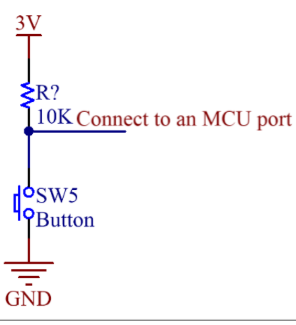
\includegraphics[width=0.4\textwidth]{graphics/button_sche.PNG}
    \caption{Cách kết nối nút nhấn đáng tin cậy}
\end{figure}

Nếu kết nối trực tiếp nút nhấn với MCU, với 16 nút nhấn sẽ phải tốn tới 16 chân của vi điều khiển, điều này khá lãng phí. Để giải quyết vấn đề này, ta có thể rút ngắn bằng việc xử lý chúng theo hàng và cột (theo ma trận). Khi đó, ta sẽ chuyển 16 nút nhấn thành 4 hàng và 4 cột (tương đương với 8 chân vi điều khiển).

Với phương pháp sử dụng IC 74HC165 ta đang dùng, ta chỉ cần kết nối 3 chân của IC với MCU, cụ thể là các chân PL, CP, Q7. IC 74HC165 hoạt động với nguyên lý sau:
\begin{itemize}
    \item Khi tín hiệu chân \textbf{PL} ở mức thấp, giá trị từ các ngõ vào D0-D7 sẽ được nạp song song vào thanh ghi trong IC.
    \item Khi tín hiệu chân \textbf{PL} ở mức cao và phát hiện cạnh lên ở chân \textbf{CP}, các giá trị bên trong thanh ghi sẽ được dịch và tín hiệu \textbf{Q7} sẽ lần lượt thể hiện các giá trị trong thanh ghi.
\end{itemize}
\begin{figure}[!htbp]
    \centering
    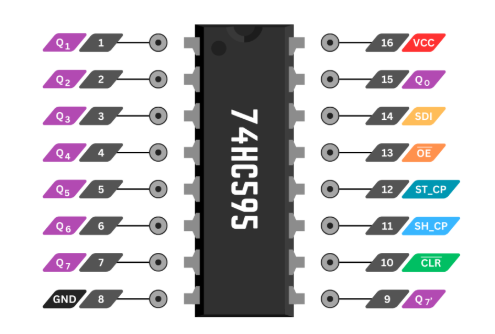
\includegraphics[width=0.7\textwidth]{graphics/ic_74HC165.PNG}
\end{figure}

Cơ chế hoạt động của 74HC165 có thể được điều khiển bởi giao tiếp SPI. Tín hiệu SCK, MISO của MCU sẽ lần lượt được kết nối với chân \textbf{CP} và \textbf{Q7} của IC. \textbf{BTN\_LOAD} sẽ được cấu hình thành \textbf{GPIO\_OUTPUT}